\section{Conclusion}
\label{conclusion}

\begin{figure}[t]
	\centering
	\subfigure{
		\centering
		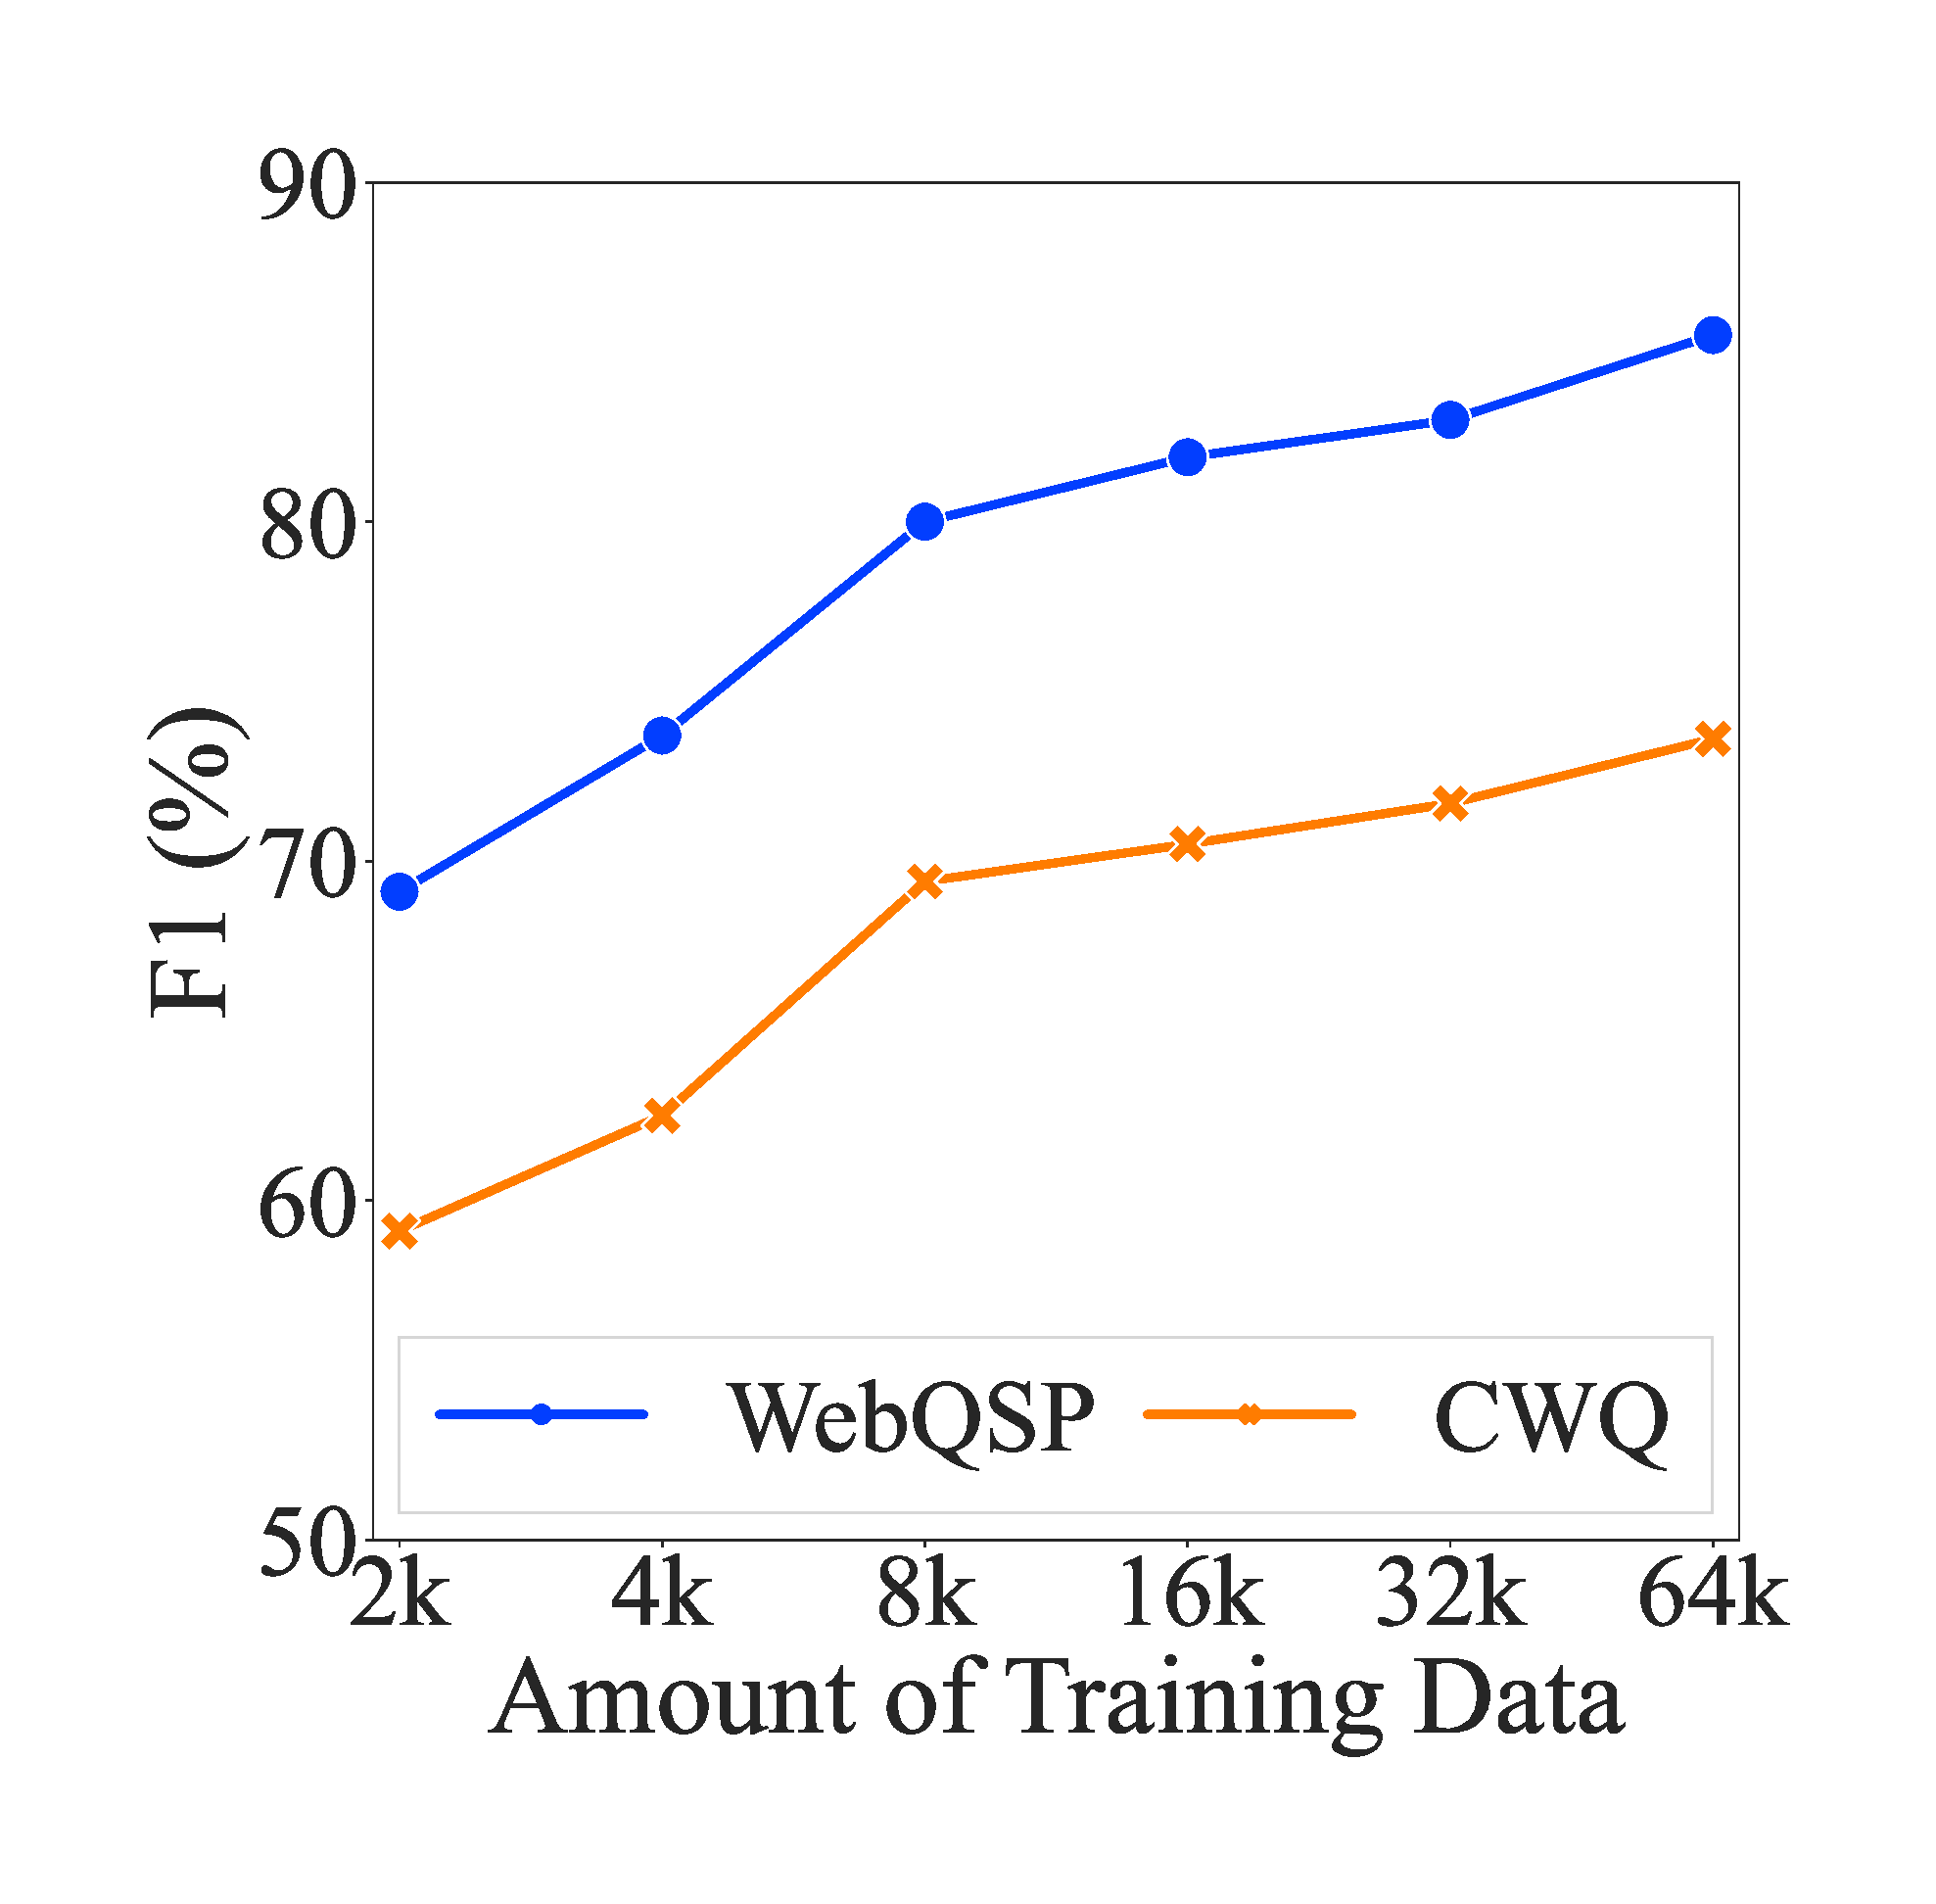
\includegraphics[width=0.22\textwidth]{resource/kgqa_line.pdf}
	}
	\subfigure{
		\centering
		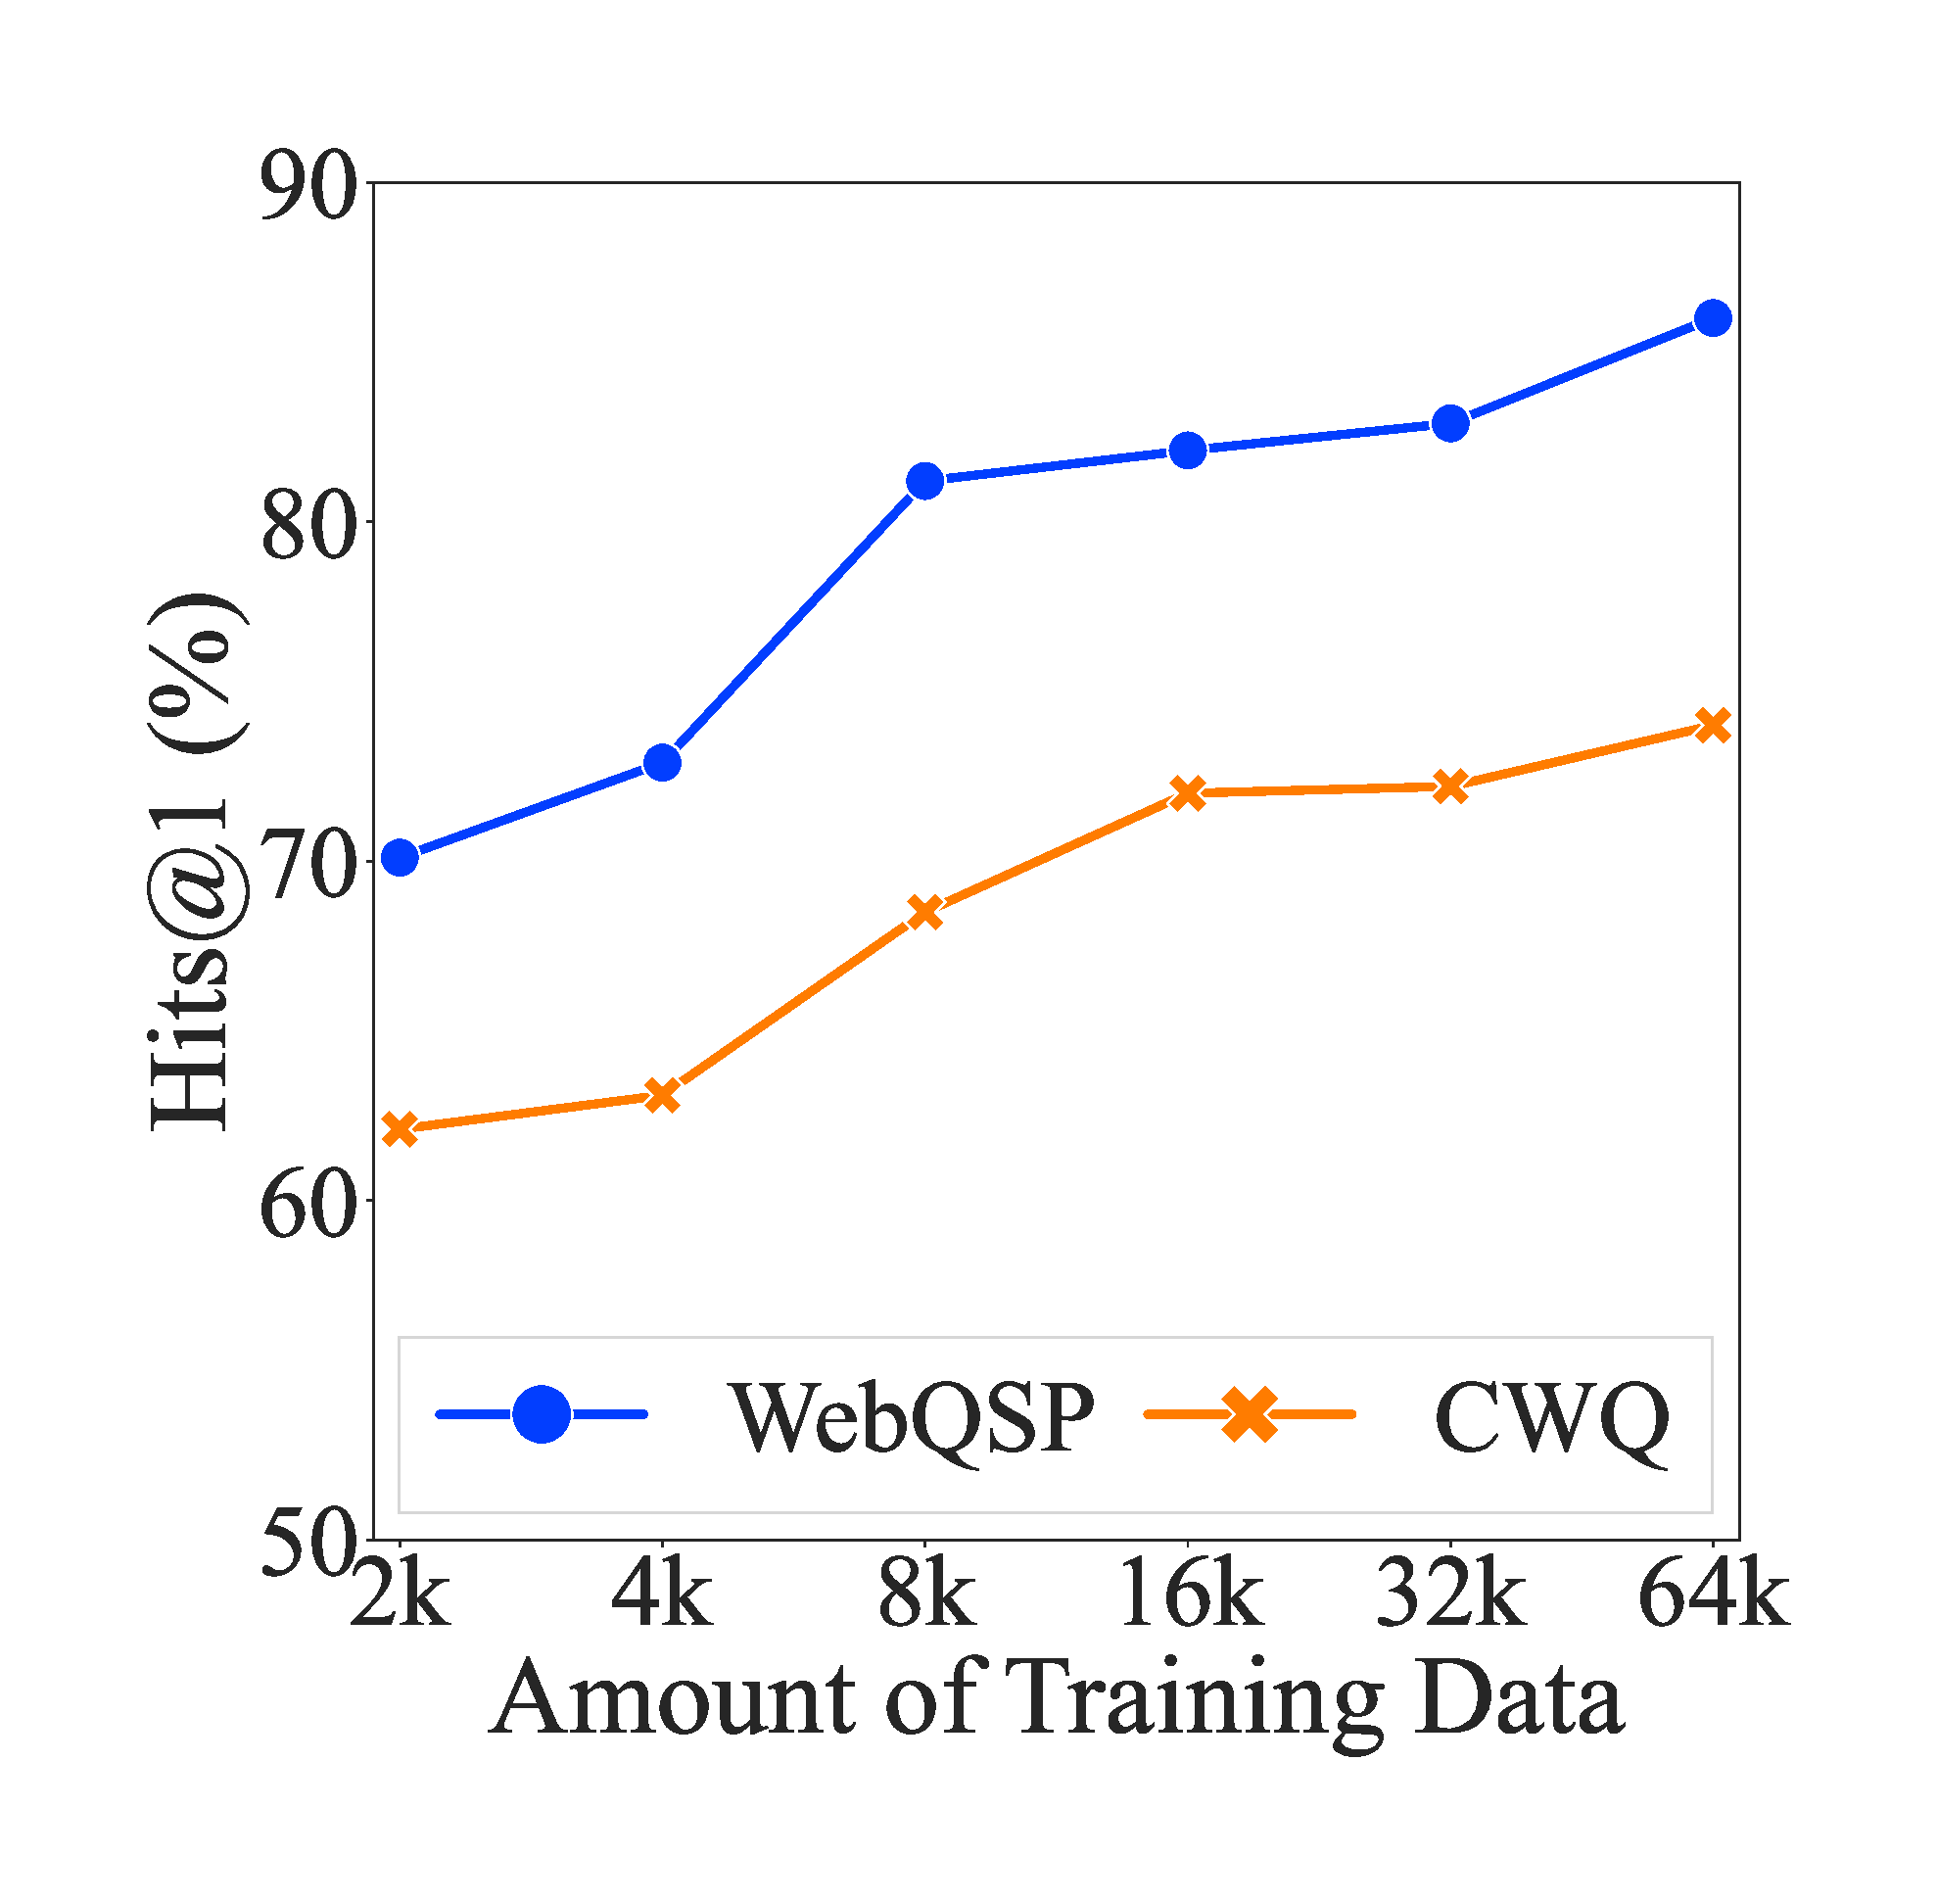
\includegraphics[width=0.22\textwidth]{resource/kgqa_hits1_line.pdf}
	}
	\centering
	\caption{The F1~(Left) and Hits@1~(Right) scores of KG-Agent on the test set of WebQSP and CWQ with a various amount of instruction tuning data.}
	\label{fig:amount}
	% \vspace{-0.2cm}
\end{figure}

In this work, we proposed an autonomous agent framework to synergize LLMs and KGs to perform complex reasoning over KG, namely KG-Agent. In our approach, we first curated a toolbox for KG, consisting of three types of tools to support the typical operations when reasoning on KG. Then, we developed an autonomous iteration mechanism based on tool selection and memory updation that integrates the LLM, multifunctional toolbox, KG-based executor, and knowledge memory, for reasoning over KG. Next, we leveraged existing KGQA datasets to synthesize the code-based instruction tuning dataset. Finally, with only 10K tuning samples, we implemented the autonomous agent relying on the smaller 7B LLM, which mostly outperforms state-of-the-art baselines based on full-data tuning or larger LLMs. In future work, we will consider extending our framework to deal with more types of structured data, \eg databases and tables.
